\begin{center}
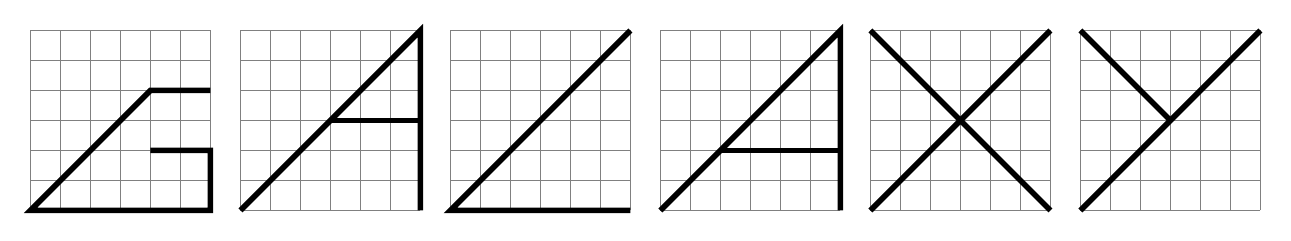
\begin{tikzpicture}[x=0.15in,y=0.15in] 
\begin{scope}[shift={(0,0)}] %GOOD G
\fill[white] (0,0) rectangle (6,6);
\draw[step=1,thin,gray] (0,0) grid (6,6);
\draw[line width=2pt] (4,2) -- (6,2) -- (6,0) -- (0,0) -- (4,4) -- (6,4);
\end{scope}
\begin{scope}[shift={(7,0)}] %GOOD A(1)
\fill[white] (0,0) rectangle (6,6);
\draw[step=1,thin,gray] (0,0) grid (6,6);
\draw[line width=2pt] (0,0) -- (6,6) -- (6,0);
\draw[line width=2pt] (3,3) -- (6,3);
\end{scope}
\begin{scope}[shift={(14,0)}] %GOOD L
\fill[white] (0,0) rectangle (6,6);
\draw[step=1,thin,gray] (0,0) grid (6,6);
\draw[line width=2pt] (6,0) -- (0,0) -- (6,6);
\end{scope}
\begin{scope}[shift={(21,0)}] %GOOD A(2)
\fill[white] (0,0) rectangle (6,6);
\draw[step=1,thin,gray] (0,0) grid (6,6);
\draw[line width=2pt] (0,0) -- (6,6) -- (6,0);
\draw[line width=2pt] (2,2) -- (6,2);
\end{scope}
\begin{scope}[shift={(28,0)}] %GOOD X
\fill[white] (0,0) rectangle (6,6);
\draw[step=1,thin,gray] (0,0) grid (6,6);
\draw[line width=2pt] (0,0) -- (6,6);
\draw[line width=2pt] (0,6) -- (6,0);
\end{scope}
\begin{scope}[shift={(35,0)}] %GOOD Y
\fill[white] (0,0) rectangle (6,6);
\draw[step=1,thin,gray] (0,0) grid (6,6);
\draw[line width=2pt] (0,0) -- (6,6);
\draw[line width=2pt] (0,6) -- (3,3);
\end{scope}
\end{tikzpicture}
\end{center}
